\documentclass[a4paper, 11pt]{article}

\usepackage[utf8]{inputenc}   
\usepackage[T1]{fontenc}       


\usepackage{amsmath}           
\usepackage{amssymb}           
\usepackage{amsthm}           
\usepackage{mathtools} 
\usepackage{pgfplots}
\pgfplotsset{compat=1.17}

\usepackage{graphicx}          % Per includere immagini
\usepackage{float}             % Per posizionare le figure esattamente dove vuoi (H)


\usepackage{geometry}          % Gestione margini
\geometry{a4paper, margin=2.5cm}
\usepackage{hyperref}          % Link cliccabili e segnalibri nel PDF

% --- Metadati Documento ---
\title{Kernel generalization error under isotropic distribution}
\author{}
\date{Week 1}

\begin{document}
	
\maketitle

\section{Setting}
Let us consider a kernel $K(\vec x, \vec y)$ where $\vec x \in \mathbb{R}^d$. We will only consider inner-product kernels (or dot-product kernels):
$$
K(\vec x, \vec y) = h(\langle \vec x, \vec y \rangle)
$$
where $h \in \mathcal{C}^{\infty}$. This way, we should be able to express $h$ as a power series $h(t) = \sum_m^\infty h_m t^m$.

When studying the generalization error of a kernel machine, we are interested in identifying the spectrum of the operator $T$:
$$
T f(x) = \int d^d \vec y \>  p(\vec y) K(\vec x, \vec y) f(\vec y)
$$
where $p(\vec x)$ is the probability distribution of the data. In this first report, we are going to consider a gaussian isotropic case where $p  = \mathcal{N}(0, \mathbb{I}_d)$

The operator $T$ is linear, symmetric and compact (!), $T : L_2(p) \to L_2(p)$ and can be diagonalized:
$$
\int d^d \vec y \>  p(\vec y) K(\vec x, \vec y) f_\beta(\vec y) = \lambda_\beta f_\beta(\vec x)
$$
By Mercer's theorem, this is equivalent to:
$$
K(\vec x, \vec y) = \sum_i \lambda_i \varphi_i(\vec x) \varphi_i(\vec y)
$$
where $\varphi_\beta$ are an orthonormal basis of the $L_2(p)$ space. In this specific case, they can be represented through Hermite polynomials.

In general, one can show (?) the eigenvalues can be indexed through a multi-index $\beta = (\beta_1, \beta_2, \dots, \beta_d)$ yielding:
$$
K(\vec x, \vec y) = \sum_\beta \lambda_\beta He_\beta(\vec x) He_\beta(\vec y)
$$
where 
$$
He_\beta(\vec x) = \prod_i He_{\beta_i}(x_i)
$$
Using an argument of symmetry (the gaussian isotropic measure is invariant under rotation and the same goes for dot-product kernel), we should get a Mercer decomposition of the kind:
$$
K(\vec x, \vec y) = h(\langle \vec x, \vec y \rangle) = \sum_m^\infty \xi_m \sum_{|	\beta| = m} He_\beta(\vec x) He_\beta(\vec y)
$$
The full derivation for the derivation of $\xi_m$ can be found in [Paper 2]:
$$
\xi_m = h_m m! d^{-m}
$$
the degeneracies of a level $m$ is given by the possible ways of arranging $(\beta_1, \beta_2, \dots, \beta_d)$ such that $|\beta| = \beta_1 + \beta_2 + \dots + \beta_d = m$. It turns out this is equivalent to:
$$
g_m = {d+m-1 \choose m}
$$
when $d \gg 1$, $g_m  = \frac{1}{m!} d^m$
\begin{figure}
	\centering
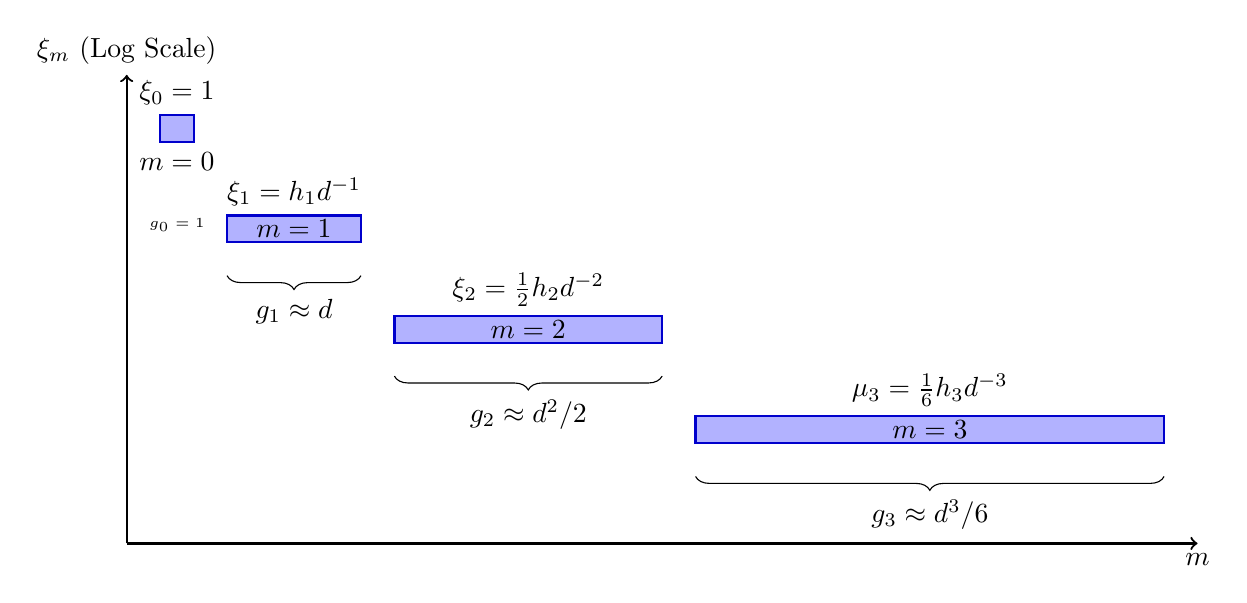
\begin{tikzpicture}[
	scale=0.85,
	level/.style={fill=blue!30, draw=blue!80!black, thick},
	tail/.style={fill=gray!30, draw=gray!80!black, dashed},
	annotation/.style={font=\small\sffamily, align=center}
	]
	
	% --- ASSI ---
	% Disegniamo un asse Y logaritmico schematico
	\draw[->, thick] (0,0) -- (0, 7) node[above] {$\xi_m$ (Log Scale)};
	\draw[->, thick] (0,0) -- (16,0) node[below] {$m$};
	
	% --- LIVELLI SPETTRALI ---
	
	% Livello 0: Bias (m=0)
	% Mu ~ 1, N ~ 1
	\draw[level] (0.5, 6) rectangle ++(0.5, 0.4);
	\node at (0.75, 5.7) {$m=0$};
	\node[above] at (0.75, 6.4) {$\xi_0 = 1$};
	\node[below, font=\tiny] at (0.75, 5) {$g_0=1$};
	
	% Livello 1: Lineare (m=1)
	% Mu ~ d^-1, N ~ d
	\draw[level] (1.5, 4.5) rectangle ++(2, 0.4);
	\node at (2.5, 4.7) {$m=1$};
	\node[above] at (2.5, 4.9) {$\xi_1 = h_1 d^{-1}$};
	% Brace per la larghezza
	\draw[decorate,decoration={brace,amplitude=5pt,mirror}] (1.5,4) -- (3.5,4) 
	node[midway,below=5pt] {$g_1 \approx d$};
	

	\draw[level] (4.0, 3.0) rectangle ++(4, 0.4);
	\node at (6.0, 3.2) {$m=2$};
	\node[above] at (6.0, 3.4) {$\xi_2=\frac{1}{2}h_2 d^{-2}$};
	\draw[decorate,decoration={brace,amplitude=5pt,mirror}] (4.0,2.5) -- (8.0,2.5) 
	node[midway,below=5pt] {$g_2 \approx d^2/2$};

	\draw[level] (8.5, 1.5) rectangle ++(7, 0.4);
	\node at (12, 1.7) {$m=3$};
	\node[above] at (12, 1.9) {$\mu_3 = \frac{1}{6}h_3d^{-3}$};
	\draw[decorate,decoration={brace,amplitude=5pt,mirror}] (8.5,1) -- (15.5,1) 
	node[midway,below=5pt] {$g_3 \approx d^3/6$};
	

\end{tikzpicture}
\end{figure}


NUMERICAL PLOTS CON EMPIRICAL DIAGONALIZATION

\section{Kernel error, $\lambda = 0$}
From Paper1, we know that the kernel generalization error is given once we compute the quantity $\nu$ defined through the self-consistency equation:
\begin{equation}
	n - \frac{\lambda}{\nu} = Tr(\Sigma (\Sigma + \mathbb{I}\nu)^{-1}) = df(\nu)
	\label{eq:paper1Kernel}
\end{equation}
where $\Sigma$ is the diagonal matrix of the eigenvalues of $k(\vec x, \vec y)$. In this work, we will use the following scaling:
$$
n = \alpha d^\kappa
$$
that is, $n \sim O(d^\kappa)$ where $\kappa$ quantifies the sample complexity and $\alpha$ is a constant (of order 1). We will consider a case where $d, n \to \infty$ while $\alpha$ remains finite.

\subsection{Computation for $\nu$}
Take Eq.\ref{eq:paper1Kernel} and substitute $\lambda = 0$ and $n = \alpha d^\kappa$:
\begin{equation}
	\alpha = d^{-\kappa} df(\nu) = d^{-\kappa} \sum_i^\infty \frac{\lambda_i}{\lambda_i + \nu}
\end{equation}
We know that in the isotropic case the eigenvalues are distributed in degenerate shells, hence:
\begin{equation}
	\alpha = d^{-\kappa} \sum_m^\infty g_m \frac{\xi_m}{\xi_m + \nu} = d^{-\kappa} \sum_m^\infty \frac{d^m}{m!} \frac{h_m m! d^{-m}}{h_m m! d^{-m} + \nu}
\end{equation}
Let's define $h_m m! = \delta_m$. In all usual cases, $\delta_m \sim O(1)$ w.r.t $m$ (for polynomials, it eventually becomes zero. For regular functions like the exponential, $d_m = 1, \forall m$). The trick here is to work under the thermodynamic limit dividing the sum in three terms:
\begin{equation}
	\begin{aligned}
			\alpha &= d^{-\kappa} \sum_m^\infty \frac{d^m}{m!} \frac{\delta_m d^{-m}}{\delta_m d^{-m} + \nu} = \\
			&= d^{-\kappa}\left( \sum_{m = 0}^{k-1} \frac{d^m}{m!} \frac{\delta_m d^{-m}}{\delta_m d^{-m} + \nu} + \frac{d^\kappa}{\kappa!} \frac{\delta_\kappa d^{-\kappa}}{\delta_\kappa d^{-\kappa} + \nu} + \sum_{m = k+1}^{\infty} \frac{d^m}{m!} \frac{\delta_m d^{-m}}{\delta_m d^{-m} + \nu}\right)
	\end{aligned}
\end{equation}
To make things work, we have to make an ansatz. We will guess:
$$
\nu = \xi d^{-\kappa}
$$
PLOT NUMERICI PER CONFERMARE ANSATZ
Let's consider the three terms separately:
\begin{itemize}
	\item \textbf{First term}:
	\begin{equation}
		d^{-\kappa} \sum_{m = 0}^{k-1} \frac{d^m}{m!} \frac{\delta_m d^{-m}}{\delta_m d^{-m} + \xi d^{-\kappa}}
	\end{equation}
	Fix a value for $0 \leq m \leq k-1$. Then the eigenvalue term:
	\begin{equation}
		 \frac{\delta_m d^{-m}}{\delta_m d^{-m} + \xi d^{-\kappa}} = \frac{1}{1+ \frac{\xi}{\delta_m}d^{m-k}} \xrightarrow{d \gg 1, m < k} 1
	\end{equation}
	Since $\xi$ is independent of $d$ by construction and $\delta_m$ is of order 1 with respect to $m$. 
	
	The first term then becomes:
		\begin{equation}
		\sum_{m = 0}^{\kappa-1} \frac{d^m}{m!} = \sum_{m = 0}^{\kappa-1} \frac{d^{m-\kappa}}{m!} \xrightarrow{d \gg 1} 0
	\end{equation}
	
	\item \textbf{Central term}: This is easy, as it evaluates to something of order 1:
	\begin{equation}
		d^{-\kappa}\frac{d^\kappa}{\kappa!} \frac{\delta_\kappa d^{-\kappa}}{\delta_\kappa d^{-\kappa} + \xi d^{-\kappa}} = \frac{1}{\kappa !} \frac{\delta_k}{\delta_k + \xi}
	\end{equation}
	\item \textbf{Third term}: Again, we write
	\begin{equation}
		d^{-\kappa} \sum_{m = k+1}^{\infty} \frac{d^m}{m!} \frac{\delta_m d^{-m}}{\delta_m d^{-m} + \xi d^{-\kappa}}
	\end{equation}
	Fix a value for $m > \kappa$. Then the eigenvalue term:
	\begin{equation}
		\frac{\delta_m d^{-m}}{\delta_m d^{-m} + \xi d^{-\kappa}} = \frac{1}{1+ \frac{\xi}{\delta_m}d^{m-k}} \approx \frac{\delta_m}{\xi} d^{\kappa - m}  \text{      when   } d \gg 1
	\end{equation}
	This term alone converges to $0$ but it needs to be considered inside the summation:
	\begin{equation}
		d^{-\kappa} \sum_{m = k+1}^{\infty} \frac{d^m}{m!} \frac{\delta_m d^{-m}}{\delta_m d^{-m} + \xi d^{-\kappa}} \approx d^{-\kappa} \sum_{m = k+1}^{\infty} \frac{d^m}{m!} \frac{\delta_m}{\xi} d^{\kappa - m} = \sum_{m = k+1}^{\infty}\frac{\delta_m}{\xi m!}
	\end{equation}
	We will define:
	$$
	l(\kappa) = \sum_{m = k+1}^{\infty}\frac{\delta_m}{m!}
	$$
	and the third term can be rewritten as $\frac{l(\kappa)}{\xi}$\footnote{If $\delta_m$ is of order 1, then this function should always converge, approfondisci meglio}
\end{itemize}
Putting all of this together, we get:
\begin{equation}
	\alpha = \frac{1}{\kappa !} \frac{\delta_k}{\delta_k + \xi} + \frac{l(\kappa)}{\xi}
\end{equation}
Let's solve for $\xi$:
\begin{equation}
	\xi = \xi(\alpha, \kappa)=\frac{1}{2\alpha}\left[\left(\frac{1}{\kappa!}\delta_\kappa + l(\kappa)-\alpha \delta_\kappa\right)+\sqrt{\left(\frac{1}{\kappa!}\delta_\kappa + l(\kappa)-\alpha \delta_\kappa\right)^2+4\alpha l(\kappa) \delta_\kappa}\right]
\end{equation}
which is independent of $d$, confirming our scaling ansatz. Finally, one has:
\begin{equation}
	\nu = \xi(\alpha, \kappa) d^{-\kappa}
	\label{eq:nu}
\end{equation}

NUMERICAL FIGURE DISPLAYING THE PERFECT AGREEMENT WITH A NUMERICAL SOLVER
\subsection{Extreme cases}
When using an exponential kernel, one has $\delta_\kappa = 1, \forall \kappa$ (note that $\delta_\kappa$ is just the derivative of the $h$ function evaluated at $0$.)

What happens when we use a polynomial kernel of degree $\kappa_0$? This essentialy means $\delta_m = 0 \> \> \forall m \geq \kappa_0$. There can be two cases:
\begin{itemize}
	\item When $\kappa < \kappa_0$, then $\delta_\kappa \neq 0$ and $l(\kappa) \neq 0$, hence we can safely use Eq.\ref{eq:nu}
	\item When $\kappa > \kappa_0$, then $\delta_\kappa = 0$ and $l(\kappa) = 0$. This implies $\nu = 0$. [?? BIAS NULLO MA VARIANZA MAL DEFINITA]
\end{itemize}
\subsection{Computation for $Var(\alpha, \kappa)$}
Again, from Paper 1 (but also Cheng, Montanari) we have:
\begin{equation}
	V(\alpha, \beta, \lambda = 0) = V = \sigma_\epsilon^2 \frac{Tr(\Sigma^2(\Sigma+\nu)^{-2})}{n-Tr(\Sigma^2(\Sigma+\nu)^{-2})} = \frac{\frac{1}{n}Tr(\Sigma^2(\Sigma+\nu)^{-2})}{1-\frac{1}{n}Tr(\Sigma^2(\Sigma+\nu)^{-2})} = \frac{\tau}{1-\tau}
\end{equation}
Let's compute $\tau$, the procedure is similar to the one we have seen above.
\begin{equation}
	\tau = \frac{1}{n}Tr(\Sigma^2(\Sigma+\nu)^{-2}) = \frac{1}{n} \sum_m g_m \frac{\xi_m^2}{(\xi_m + \nu)^2} 
\end{equation}
As usual, we divide the summation in three pieces and let $n = \alpha d^{\kappa}$.
\begin{equation}
	\tau = \alpha^{-1} d^{-\kappa} \sum_{m=0}^{k-1} g_m \frac{\xi_m^2}{(\xi_m + \nu)^2} + \alpha^{-1} d^\kappa g_\kappa \frac{\xi_\kappa^2}{(\xi_\kappa + \nu)^2} + \alpha^{-1} d^\kappa \sum_{m=k+1}^{\infty} g_m \frac{\xi_m^2}{(\xi_m + \nu)^2}
\end{equation}
\begin{itemize}
	\item \textbf{First term}: 
	\begin{equation}
		\begin{aligned}
			\alpha^{-1} d^{-\kappa} \sum_{m=0}^{k-1} g_m \frac{\xi_m^2}{(\xi_m + \nu)^2} &= \alpha^{-1}d^{-\kappa} \sum_{m=0}^{k-1} \frac{1}{m!} d^{m} \frac{\delta_m^2 d^{-2m}}{\xi^2 d^{-2\kappa} + \delta_m^2 d^{-2m} + \delta_m \xi d^{-m-k}} = \\
			&= \alpha^{-1} \sum_{m=0}^{k-1} \frac{1}{m!} \frac{\delta_m^2 d^{-\kappa-m}}{\xi^2 d^{-2\kappa} + \delta_m^2 d^{-2m} + \delta_m \xi d^{-m-k}} = \\
			&= \alpha^{-1} \sum_{m=0}^{k-1} \frac{1}{m!} \frac{\delta_m^2}{\xi^2 d^{m-\kappa} + \delta_m^2 d^{-m+\kappa} + \delta_m \xi} \underset{d \gg 1}{\approx} \\
			&\underset{d \gg 1}{\approx} \sum_{m = 0}^{\kappa-1}\frac{1}{\alpha m!} d^{\kappa-m} \xrightarrow{d \gg 1} 0
		\end{aligned}
	\end{equation}
	Since, again, the terms $\delta_m, \xi$ are assumed to be $O(1)$ with respect to $d$.
	\item \textbf{Central term}
	\begin{equation}
		\alpha^{-1} d^{-\kappa} \frac{1}{\kappa !} d^{\kappa} \frac{\delta_\kappa^2}{(\delta_\kappa + \xi)^2} = \frac{1}{\alpha \kappa !} \frac{\delta_\kappa^2}{(\delta_\kappa + \xi)^2}
	\end{equation}
	\item \textbf{Third term}
		\begin{equation}
			\begin{aligned}
				\alpha^{-1} d^{-\kappa} \sum_{m=\kappa+1}^{\infty} g_m \frac{\xi_m^2}{(\xi_m + \nu)^2} &= \alpha^{-1} \sum_{m=\kappa+1}^{\infty} \frac{1}{m!} \frac{\delta_m^2}{\xi^2 d^{m-\kappa} + \delta_m^2 d^{-m+\kappa} + \delta_m \xi} \overset{d \gg 1}{\approx} \\
				&\overset{d \gg 1}{\approx} \alpha^{-1} \sum_{m=\kappa+1}^{\infty} \frac{1}{m!} d^{\kappa - m} \xrightarrow{d \gg 1} 0
			\end{aligned}
		\end{equation}

\end{itemize}
So for the variance, the only term that counts is the one of order $m = \kappa$. Finally, we obtain:
\begin{equation}
	\tau \approx \frac{1}{\alpha \kappa !} \frac{\delta_\kappa^2}{(\delta_\kappa + \xi(\alpha, \kappa))^2}
\end{equation}
where $\xi(\alpha, \kappa)$ can be computed as in Eq.\ref{eq:nu}. The full variance will then become:
\begin{equation}
	Var(\alpha, \kappa, \lambda = 0) = \sigma_\epsilon^2\frac{1-\tau}{\tau} = \sigma_\epsilon^2 \frac{\delta_\kappa^2}{\alpha \kappa! (\delta_\kappa + \xi)^2 - \delta_\kappa^2}
\end{equation}
[TO DO: CONDITION SUCH THAT DENOMINATOR IS POSITIVE?]
\\

[NUMERICAL PLOT OF VARIANCE SHAPE, TENDS TO ZERO AS ALPHA GROWS]

\subsection{Computation for $B(\alpha, \kappa)$}
The bias term is given by:
\begin{equation}
	B(\alpha, \kappa) = \frac{\nu^2 \langle \vec\theta, (\Sigma + \nu)^{-2} \vec\theta\rangle}{1-\tau}
	\label{eq:bias1}
\end{equation}
where $\vec\theta$ is the orthonormal decomposition of the target function $f_\star(\vec x)\in L_2(\mathcal{N}(0,\mathcal{I_d}))$. In particular, given the generalized $d$-dimensional Hermite polynomials, we can write:
\begin{equation}
	f_\star (\vec x) = \sum_{\beta \in \mathbb{N}^d} \theta_\beta He_\beta(\vec x) = \sum_{\beta \in \mathbb{N}^d} \theta_\beta  \prod_{i = 1}^{d}He_{\beta_i}(x_i) 
\end{equation}
In general, the eigendecomposition of $f_\star$ cannot be organized in degenerate levels since we are only assuming $f_\star$ is square-integrable:
$$
||f_\star||^2_{L_2} = \sum_{\beta \in \mathbb{N}^d}\theta_\beta^2 = 1
$$
but $f_\star$ may easily be not rotationally invariant (as was the case for the kernel $k(x,x')$).

Now let's compute the numeratore of Eq.\ref{eq:bias1}: 
\begin{equation}
	\begin{aligned}
		\nu^2 \langle \vec\theta, (\Sigma + \nu)^{-2} \vec\theta\rangle =  \sum_{\beta \in \mathbb{N}^d} \theta_\beta^2 \frac{\nu^2}{(\lambda_\beta + \nu)^2} = \sum_{m = 0}^\infty \frac{\nu^2}{(\xi_m+\nu)^2} \sum_{|\beta| = m} \theta_\beta^2
	\end{aligned}
\end{equation}
Let's define:
$$
\Theta(m) = \sum_{|\beta| = m} \theta_\beta^2
$$
So that finally:
\begin{equation*}
	\begin{aligned}
			\nu^2 \langle \vec\theta, (\Sigma + \nu)^{-2} \vec\theta\rangle &= \sum_{m = 0}^\infty \Theta(m) \frac{\xi^2 d^{-2k}}{(\delta_m d^{-m} + \xi d^{-k})^2} = \sum_{m = 0}^\infty \Theta(m) \frac{\xi^2 d^{-2k}}{\delta_m^2 d^{-2m} + \xi^2 d^{-2\kappa} + 2\delta_m \xi d^{-m-\kappa}} = \\
		& = \sum_{m = 0}^\infty \Theta(m) \frac{\xi^2}{\delta_m^2 d^{2(-m+\kappa)} + \xi^2 + 2\delta_m \xi d^{-m+\kappa}}
	\end{aligned}
\end{equation*}
To solve asymptotically this equation, we will perform the usual trick.
\begin{itemize}
	\item When $0 \leq m \leq \kappa$, then the terms $d^{-m+\kappa}$ and $d^{2(-m+\kappa)}$ will both diverge to infinity. Consequently, the whole fraction will converge to $0$ as $d \to \infty$. The prefactor $\Theta(m)$ is independent of $d$\footnote{Is it really? Or just O(1)?}, so the whole term goes to $0$ when $ m < \kappa$
	\item When $m = \kappa$, we obtain:
	\begin{equation}
		\Theta(\kappa)\frac{\xi^2}{(\xi+\delta_\kappa)^2}
	\end{equation}
	\item When $m > \kappa$, then the terms $d^{-m+\kappa}$ and $d^{2(-m+\kappa)}$ will both converge to $0$. We are left with:
	\begin{equation}
		\sum_{m > k} \Theta(m) \frac{\xi^2}{\delta_m^2 d^{2(-m+\kappa)} + \xi^2 + 2\delta_m \xi d^{-m+\kappa}} \approx \sum_{m > k}\Theta(m)
	\end{equation} 
	This summation here is convergent, since $||f|| = \sum_{m }\Theta(m) < \infty$
\end{itemize}

Finally, we have:
\begin{equation}
	\nu^2 \langle \vec\theta, (\Sigma + \nu)^{-2} \vec\theta\rangle = \frac{\xi^2}{(\xi + \delta_\kappa)^2}\Theta(\kappa) + \sum_{m > k}\Theta(m)
\end{equation}
This is a nice formula! Combining all together, I get:
\begin{equation}
	B(\alpha, \kappa, \vec \theta) = \frac{\frac{\xi^2}{(\xi + \delta_\kappa)^2}\Theta(\kappa) + \sum_{m > k}\Theta(m)}{1-\tau} = \frac{\frac{\xi^2}{(\xi + \delta_\kappa)^2}\Theta(\kappa) + \sum_{m > k}\Theta(m)}{1-\frac{1}{\alpha \kappa !} \frac{\delta_\kappa^2}{(\delta_\kappa + \xi)^2}} 
\end{equation}
When $\alpha \to \infty$ (a lot of data, but still scaling with $d^\kappa$), then:
$$
Var(\alpha, \kappa) \to 0
$$
$$
B(\alpha, \kappa, \vec\theta) \approx \sum_{m > k}\Theta(m)
$$
The last quantity is extremely interesting. It represents the projection of the target function $f_\star$ on the space spanned by Hermite polynomials whose degree is higher than the sample complexity $\kappa$. This is the irreducible bias, the error we cannot avoid since we do not have enough data.


ASYMPTOTIC BEHAVIOR OF $\xi, \tau$ as $\alpha \to \infty$. (both goes to $0$). 
\end{document}